% !TeX document-id = {0beb03b8-2a83-45f5-aca6-99def446a6e3}
% !TEX TS-program = pdflatexmk
\documentclass[12pt]{article}
\usepackage{a4wide}
\usepackage{amsmath,amssymb}
\usepackage{bm}
\usepackage{enumitem}
\usepackage[colorlinks]{hyperref}
\usepackage{graphicx}
\usepackage{appendix}
\usepackage{color}
\newcommand{\vect}[1]{\hat{\boldsymbol{#1}}}

\newcommand{\reporttitle}{Project Report : Lorenz system}
\newcommand{\reportauthorOne}{Melissa Aydogdu}
\newcommand{\reportauthorTwo}{Frédérique Lecourtier}
\newcommand{\reportsupervisorOne}{Christophe Prudhomme}
\newcommand{\reportsupervisorTwo}{Luca Berti}
\newcommand{\reporttype}{Coursework}

\hypersetup{
	colorlinks=true,
	linkcolor=blue,
	filecolor=magenta,      
	urlcolor=cyan,
}

\begin{document}
	\nocite{*}
	
	\begin{titlepage}

\newcommand{\HRule}{\rule{\linewidth}{0.5mm}} % Defines a new command for the horizontal lines, change thickness here

\begin{center} % Center remainder of the page


\includegraphics[width = 0.5\linewidth]{images/logo-cemosis.pdf}\\[1.5cm] 

\textsc{\Large University of Strasbourg}\\[0.5cm] 
\textsc{\large Master CSMI}\\[0.95cm] 

%----------------------------------------------------------------------------------------
%	TITLE SECTION
%----------------------------------------------------------------------------------------

\HRule \\[0.4cm]
{ \huge \bfseries \reporttitle}\\ % Title of your document
\HRule \\[1.5cm]
\end{center}
%----------------------------------------------------------------------------------------
%	AUTHOR SECTION
%----------------------------------------------------------------------------------------

%\begin{minipage}{0.4\hsize}
\begin{flushleft} \large
	\begin{minipage}{0.4\hsize}
		\textit{Authors:}\\
		\reportauthorOne\\
		\reportauthorTwo
	\end{minipage} \hfill 
	\begin{minipage}{0.4\hsize}
		\textit{Supervisors:}\\
		\reportsupervisorOne\\
		\reportsupervisorTwo
	\end{minipage}
\end{flushleft}
\vspace{4cm}
\makeatletter
Date: \@date 

\vfill % Fill the rest of the page with whitespace



\makeatother


\end{titlepage}


	
	\tableofcontents
	
	\newpage
	
	\section{Introduction}
	
	\subsection{Cemosis}
	
	This project is managed by Cemosis which is the "Centre de Modélisation et de Simulation de Strasbourg" (Strasbourg Modeling and Simulation Center). Cemosis is hosted by the Institute of Advanced Mathematical Research (IRMA) and was created in January 2013. Cemosis mainly relies currently on the team Modeling and Control of the IRMA. Their main objectives are :
	
	\begin{enumerate}[label=\textbullet]
		\item \textbf{MSO} - Modeling Simulation and Optimization
		\item \textbf{DS} -	Data Science, Big Data, Smart Data
		\item \textbf{HPC} - High Performance Computing, Parallel Computing, Cloud Computing
		\item \textbf{SI} - Signal and Image processing
	\end{enumerate}
	
	\noindent For more informations, refer to the \href{http://www.cemosis.fr/}{cemosis website}. 
	
	\subsection{Goals of the project}
	
	 The main objectives of the project are :
	 \begin{enumerate}[label=\textbullet]
	 	\item para-real method - to accelerate the simulation of ODE
	 	\item data assimilation, specially
	 	\begin{itemize}[label=-]
	 		\item understanding Kalman Filter
	 		\item understanding Ensemble Kalman Filter
	 	\end{itemize}
	 \end{enumerate}	 	
	
	\noindent For the organization we have chosen to make a Gantt diagram (section~\ref{diag}) with the different parts and the deadlines we have set (which can change during the time). The first part consists in understanding the Lorenz system and to make the implementation of the resolution, since this part is essential for the rest, we worked together during this. For the remainder of the project, we divided the work: one person will take care of the para-real algorithm and the other on the part with the data assimilation.
	
	\newpage
	
	\section{Some interesting properties of the Lorenz System}
	
	\subsection{Introduction to the system}
	
	For centuries, humans have used math and science to make predictions about the universe. Scientist were able to predict an eclipse a century in advance. We are now able to make predictions about asteroids impact in earth. But why can we only predict the weather about a week or two in advance? Why scientists cannot predict the temperature for long periods of time? There have been many times when the weather predictions the day before were completely different from the ones you expected. But it is important to know that weather prediction is a very complicated and difficult task to achieve. The complexity is strongly related to the earth's atmosphere, which can be considered as a fluid. 
	Around 1960 Edward Lorenz, an MIT meteorologist, started to work with a set of equations that represented a simplified version of the atmosphere, with 12 variables that changed over time. After two years of research, in 1963 he developed the Lorenz system, a simplified three-variable model to investigate atmospheric convection. This system defines a 3 dimensional trajectory by differential equations with 3 parameters.
	$$
	\begin{cases}
		
		x'&=\sigma(y-x) \\
		y'&=x(r-z)-y \\
		z'&=xy-bz
		
	\end{cases}
	$$
	
	\noindent Here, $x$ is proportional to the rate of convection, $y$ is related to the horizontal temperature variation, and $z$ is the vertical temperature variation.
	We have also three parameters all strictly positive:
	\begin{enumerate}[label=\textbullet]
		\item $\sigma > 0$  relates to the Prandtl number. This number is a dimensionless quantity that puts the viscosity of a fluid in correlation with the thermal conductivity.
		\item $r > 0$  relates to the Rayleigh, it is a control parameter, representing the temperature difference between the top and bottom of the tank
		\item $b > 0$ relates to the physical dimensions of the layer of fluid uniformly heated from below and cooled from above.
	\end{enumerate}
	
	\noindent We can see that this system is non-linear, because in the second differential equation( $\frac{dy}{dt}$) we can see the term $xz$ and in the third differential equation ($\frac{dz}{dt}$) we have $xy$. The three differential equations form a coupled system. 
	
	\noindent Let us now determine the fixed points of the Lorenz system. These are the points such that $X'=0$. 
	
	$$
	X'=(x',y',z')=0
	\quad \Rightarrow \quad 
	\left\{\begin{aligned}
		x'=&\sigma(y-x) &&=0 \\
		y'=&x(r-z)-y  &&=0\\
		z'=&xy-bz &&=0
	\end{aligned}\right. 
	\quad \Rightarrow \quad 
	\left\{\begin{aligned}
		&x=y \\
		&(r-1-z)x=0\\
		&x^2=bz
	\end{aligned}\right.
	$$
	
	\begin{enumerate}[label=\textbullet]
		\item If $x=0$ : \quad  $y=0$ and $z=0$.
		\item If $x\ne 0$ and $r>1$ : \quad $\left\{\begin{aligned}
			&z=r-1\\
			&x=y=\pm\sqrt{b(r-1)}
		\end{aligned}\right.
		$
	\end{enumerate}
	
	\noindent We deduce that the fixed points of the Lorenz system are: $(0,0,0)$ for all values of the parameters. And for $r>1$, there is also a pair of fixed points $(\sqrt{b(r-1)},\sqrt{b(r-1)},r-1)$ and $(-\sqrt{b(r-1)},-\sqrt{b(r-1)},r-1)$.
	
	\subsection{Lorenz Attractor}
	
	The Lorenz system is also called Lorenz Attractor. Let's try to undestand why. Lorenz discovered that an incredible structure emerges when $x(t)$ is plotted against $z(t)$: the famous butterfly wing pattern.
	\begin{center}
		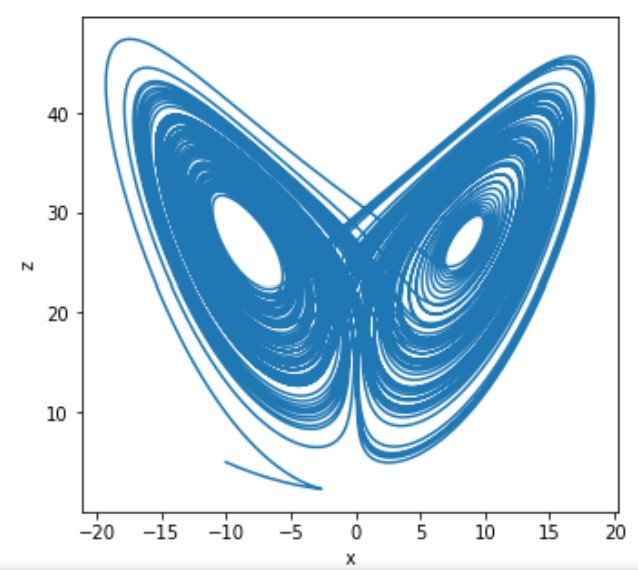
\includegraphics[width=0.5\textwidth]{"images/butterfly.jpg"}
	\end{center}
	\begin{enumerate}[label=\textbullet]
		\item The trajectory seems to cross several times, but this is just an illusion of the projection of the three dimensional trajectory on a two dimensional plane. In 3D, there are no crossings!
		\item The number of circuits made on either side varies unpredictably from one cycle to the next. The sequence of the number of circuits in each lobe has many of the characteristics of a random sequence!
		\item When the trajectory is viewed in 3 dimensions, it appears to settle onto a thin set that looks like a pair of butterfly wings. We call this attractor a strange attractor and it can be shown schematically as :
		\begin{center}
			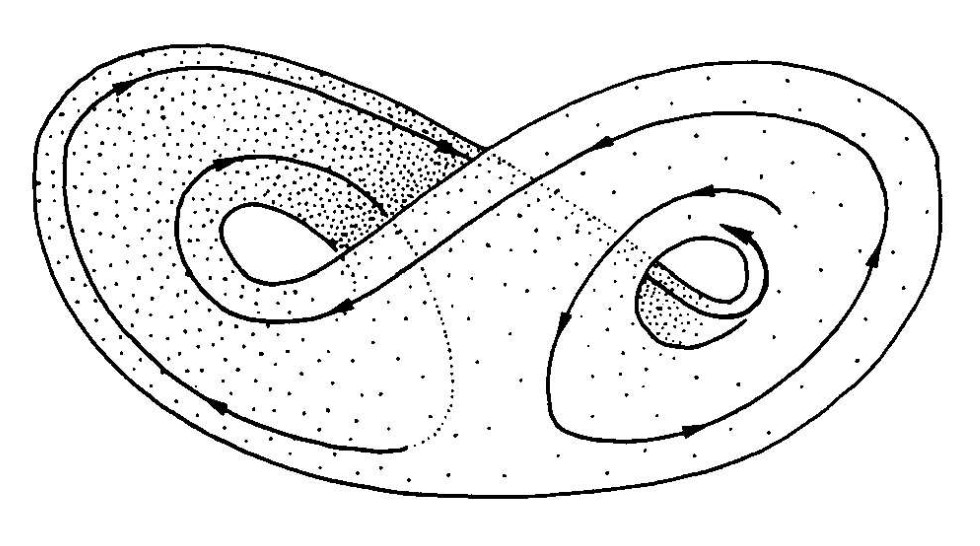
\includegraphics[width=0.5\textwidth]{"images/butterfly3D.jpg"}
		\end{center}
	\end{enumerate}
	
	\noindent The uniqueness theorem\cite{lecture6} means that trajectories cannot cross or merge, hence the two surfaces of the strange attractor can only appear to merge. Lorenz concluded that “there is an infinite
	complex of surfaces” where they appear to merge. Today this “infinite complex of surfaces” would be called a fractal, which is a set of points with zero volume but infinite surface area.
	
	\noindent The term attractor is also difficult to define in a rigorous way. Loosely, an attractor is a set of points to which all neighbouring trajectories converge. Stable fixed points and
	stable limit cycles are examples. Nobody has yet proved that the Lorenz attractor is truly an attractor. Finally we define a strange attractor to be an attractor that exhibits sensitive dependence on initial conditions\cite{lecture6}.
	
	\subsection{Chaos theory}
	
	In 1961, Lorenz was working with a simplified system that represented the atmosphere, with 12 variables. A computer was used to calculate the values for each instant by applying the equations to the values from the previous moment. In some cases, Lorenz’s team needed to re-start the simulation. Since the equations was the same, they expected to see the same results but sometimes they didn’t. At first, they thought that the problem was coming from the computer, but actually the error came from the fact that the computer was storing numbers with six decimal places but it was only printing the number with 3 decimal places, so the values that Lorenz put into the computer had tiny errors. So he discovered that in some systems, tiny changes in the initial conditions can lead to big changes in time.
	
	\noindent This effect was later named "butterfly effect". The "butterfly effect" refers to a system that is very sensitive to the initial condition, which is why these systems are very difficult to predict over time. This idea gave birth to the notion of a butterfly flapping its wings in a region of the world and causing a tornado.
	The Lorenz equations are a chaotic system, which means that this type of system is roughly defined by sensitivity to initial conditions: infinitesimal differences in initial conditions of the system result in large differences in behavior.
	
	\section{Numerical resolution with different methods}
	
	We consider $f : [0; T] \times \mathbb{R}^n \rightarrow \mathbb{R}^n$ a continuous function. For $X_0\in \mathbb{R}^n$, the problem is to find  $X\in C^1([0,T],\mathbb{R}^n)$ a solution for the differential equation:
	
	$$\left\{\begin{aligned}
		X'&=f(t,X) \\
		X(0)&=X_0
	\end{aligned}\right.$$
	
	\noindent To solve the Lorenz problem we will have:
	
	$$X'=\begin{pmatrix}
		x' \\
		y' \\
		z'
	\end{pmatrix}, \quad X=\begin{pmatrix}
		x \\
		y \\
		z
	\end{pmatrix} \quad et \quad f(t,X)=\begin{pmatrix}
		\sigma(y-x) \\
		x(r-z)-y \\
		xy-bz
	\end{pmatrix}$$
	
	\noindent After discretizing the problem in time, we can implement different methods to solve the ODE. The methods are the following and will be described in more detail in the following parts: explicit Euler, implicit Euler and Runge Kutta (order 4). We will also use a scipy function and finally compare all our methods.
	
	\subsection{Discretization}
	
	To solve the problem, we will use the finite difference method. We will start by slicing the interval $[0,T]$ in $N+1$ discretization points (so $N$ intervals). Let $t_n=n\Delta t$ the discretization timed with $\Delta t=T/N$ the times step. Then, we denote by $X_n=X(t_n)$ the discretization points. So for $n=\{0,\dots,N\}$, we will have:
	
	$$\left\{\begin{aligned} 
		x_n&=x(t_n)=x(n\Delta t) \\
		y_n&=y(t_n)=y(n\Delta t) \\
		z_n&=z(t_n)=z(n\Delta t)
	\end{aligned}\right.$$
	
	\noindent By Taylor's theorem, we get :
	
	$$\begin{aligned}
		&&X(t+\Delta t)&=X(t)+\Delta t X'(t) + O(\Delta t^2) \\
		\Rightarrow&& \quad X'(t)&=\frac{X(t+\Delta t)-X(t)}{\Delta t} + O(\Delta t) \\
		\Rightarrow&& \quad \partial_t X_n&\approx\frac{X_{n+1}-X_n}{\Delta t} \\
	\end{aligned}
	$$	
	
	\subsection{Explicit Euler}
	
	The explicit Euler method is written :
	
	$$X_{n+1}=X_n+\Delta t f(t_n,X_n)$$
	
	\noindent which will give us:
	
	$$\left\{\begin{aligned} 
		x_{n+1}&=\sigma\Delta t y_n+(1-\sigma\Delta t) x_n \\
		y_{n+1}&=\Delta t x_n(r-z_n)(1-\Delta t)y_n \\
		z_{n+1}&=\Delta t x_ny_n+(1-b\Delta t)z_n
	\end{aligned}\right.$$
	
	\subsection{Implicit Euler}
	
	The implicit Euler method is written :
	
	$$X_{n+1}=X_n+\Delta t f(t_{n+1},X_{n+1})$$
	
	\noindent which will give us:
	
	$$\left\{\begin{aligned} 
		x_{n+1}&=x_n+\Delta t\sigma(y_{n+1}-x_{n+1}) \\
		y_{n+1}&=y_n+\Delta t x_{n+1}(r-z_{n+1})-y_{n+1} \\
		z_{n+1}&=z_n+\Delta tx_{n+1}y_{n+1}-\Delta tbz_{n+1}
	\end{aligned}\right.$$
	
	\begin{enumerate}[label=\textbullet]
		\item First, we isolate the $n+1$ terms on the left and the $n$ terms on the right:
		
		$$\left\{\begin{aligned} 
			(1+\Delta t\sigma)x_{n+1}-\Delta t\sigma y_{n+1}&=x_n \\
			-\Delta t(r-z_{n+1})x_{n+1}+(1+\Delta t)y_{n+1}&=y_n \\
			-\Delta ty_{n+1}x_{n+1}+(1+\Delta tb)z_{n+1}&=z_n
		\end{aligned}\right.$$
		
		\item We can then linearize the terms 
		
		$$\begin{aligned}
			x_{n+1}y_{n+1}&\approx x_{n+1,k+1}y_{n+1,k} \\
			x_{n+1}z_{n+1}&\approx x_{n+1,k+1}z_{n+1,k}
		\end{aligned}$$ 		
		\noindent Then, we get :
		
		$$\left\{\begin{aligned} 
			(1+\Delta t\sigma)x_{n+1,k+1}-\Delta t\sigma y_{n+1,k+1}&=x_n \\
			-\Delta t(r-z_{n+1,k})x_{n+1,k+1}+(1+\Delta t)y_{n+1,k+1}&=y_n \\
			-\Delta ty_{n+1,k}x_{n+1,k+1}+(1+\Delta tb)z_{n+1,k+1}&=z_n
		\end{aligned}\right.$$
		
		\item We can then put in matrix form  $M(X_{n+1,k})X_{n+1,k+1}=X_n$ with :
		
		$$M(X_{n+1,k})=\begin{pmatrix}
			1+\Delta t\sigma & -\Delta t\sigma & 0 \\
			-\Delta t(r-z_{n+1,k}) & 1+\Delta t & 0 \\
			-\Delta ty_{n+1,k} & 0 & 1+\Delta tb
		\end{pmatrix},$$
		$$X_{n+1,k+1}=\begin{pmatrix}
			x_{n+1,k+1} \\
			y_{n+1,k+1} \\
			z_{n+1,k+1}
		\end{pmatrix} \quad et \quad X_n=\begin{pmatrix}
			x_n \\
			y_n \\
			z_n
		\end{pmatrix} $$
	\end{enumerate}

	\noindent We make a loop on the k iterator until we have :
	
	$$\frac{||x_{n+1}^{k+1}-x_{n+1}^k||}{||x_{n+1}^k||}$$
	
	\subsection{Runge Kutta}
	
	\begin{enumerate}[label=\textbullet]
		\item \textbf{Runge Kutta (order 4) :} \\
		The Runge Kutta method of order 4 is written :
		
		$$X_{n+1}=X_n+\frac{\Delta t}{6}\left(K_1+2K_2+2K_3+K_4\right)$$
		
		\noindent where 
		
		$$\left\{\begin{aligned}
			K_1&=f(t_n,X_n) \\
			K_2&=f\left(t_n+\frac{\Delta t}{2},X_n+\frac{1}{2} K_1\Delta t\right) \\
			K_3&=f\left(t_n+\frac{\Delta t}{2},X_n+\frac{1}{2} K_2\Delta t\right) \\
			K_4&=f\left(t_n+\Delta t,X_n+K_3\Delta t\right)
		\end{aligned}\right.$$
		\item \textbf{Scipy function :} \href{https://docs.scipy.org/doc/scipy/reference/generated/scipy.integrate.solve_ivp.html#scipy.integrate.solve_ivp}{scipy.integrate.solve\_ivp} \\
		This function solve an initial value problem for a system of ODEs. We can chose the method used by the argument "method" which is by default RK45. 
	\end{enumerate}
	
	\subsection{Comparing methods}
	
	\begin{enumerate}[label=\textbullet]
		\item First, we had to implement a function allowing to plot a 2D graph representing x versus y, then a 2D graph representing x versus z and finally a 3D graph of the solution. Then, we implemented the different methods described above and we checked visually that they worked correctly. Here are the graphs obtained with the following parameters :
		\begin{center}
			$\sigma=10,\quad \beta=8/3 \quad r=9/10$ \\
			$X_0=(-10,10,5)$ \\
			$N=5000, \quad T=100$
		\end{center}
		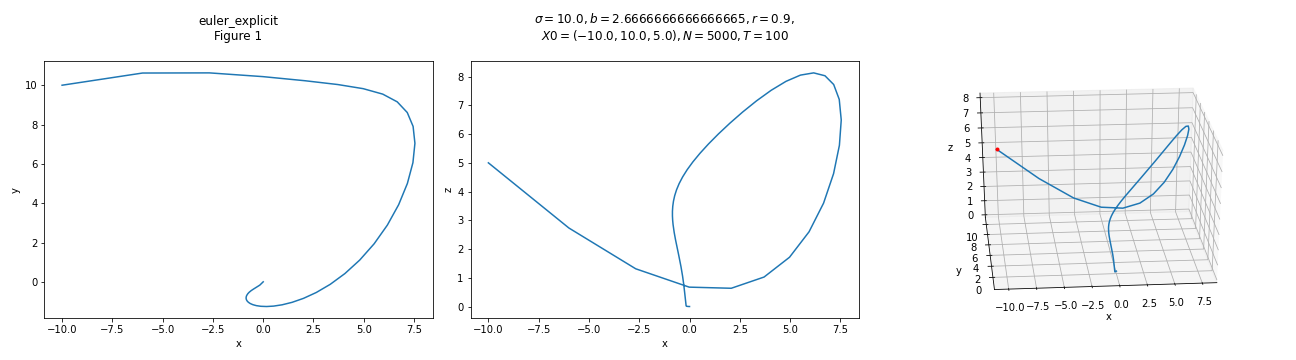
\includegraphics[width=\textwidth]{"images/euler_explicit.png"}
		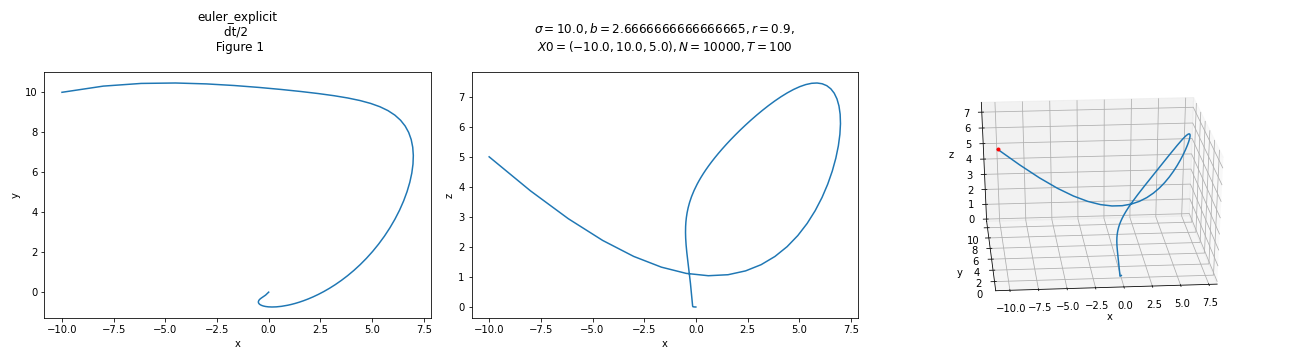
\includegraphics[width=\textwidth]{"images/euler_explicit_dt2.png"}
		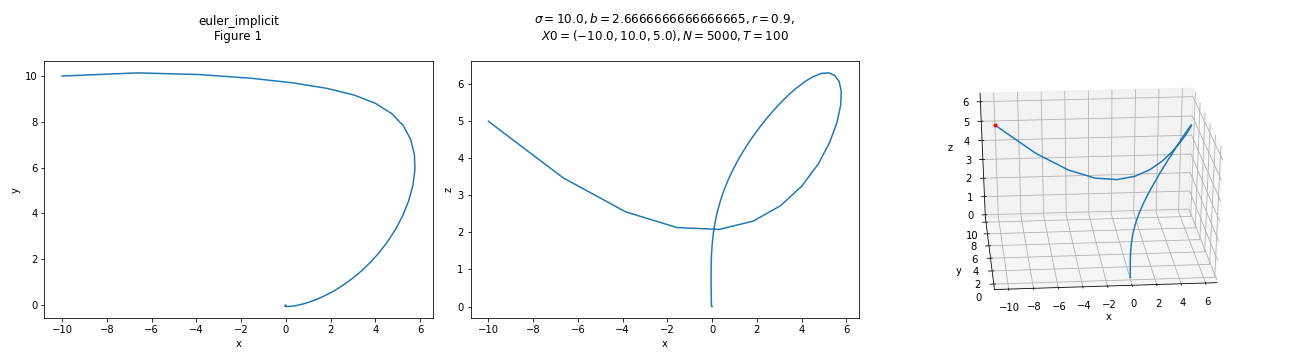
\includegraphics[width=\textwidth]{"images/euler_implicit.png"}
		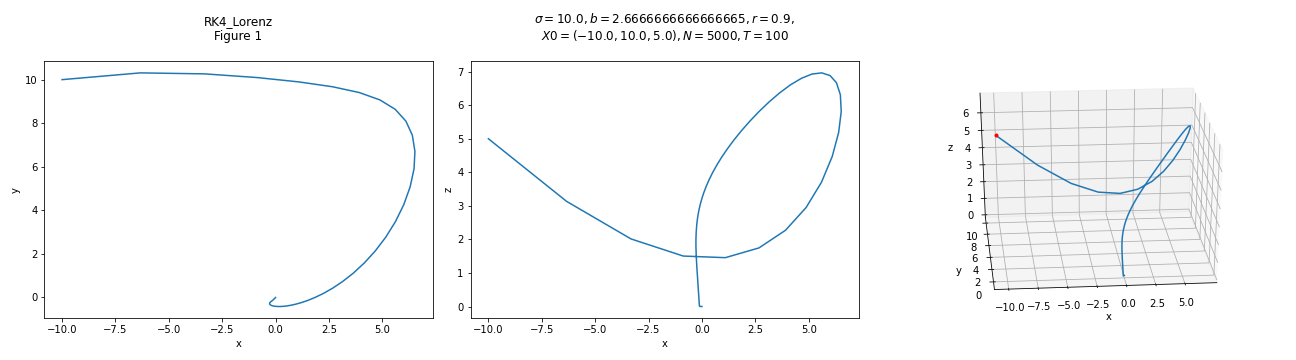
\includegraphics[width=\textwidth]{"images/RK4_Lorenz.png"}
		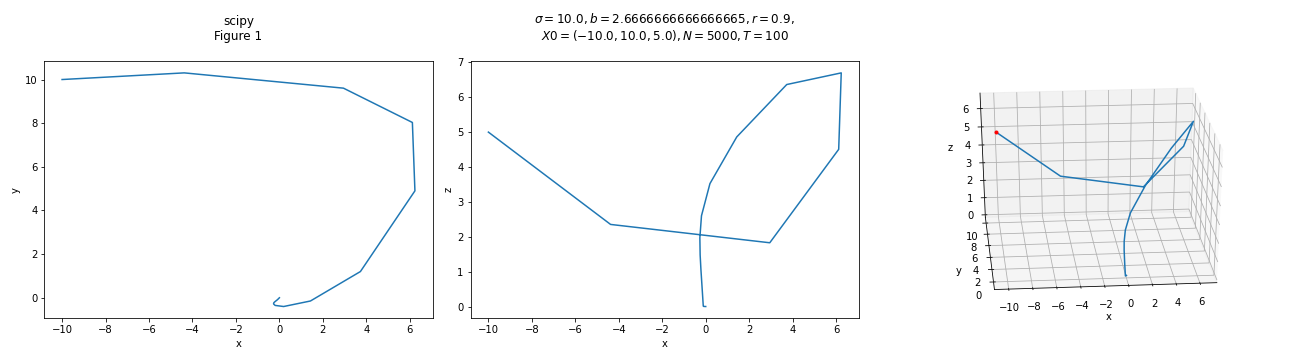
\includegraphics[width=\textwidth]{"images/scipy.png"}
		\item Then, we compared the execution times of these different methods (until $T=100$). Here is what we get with the same parameters : \\
		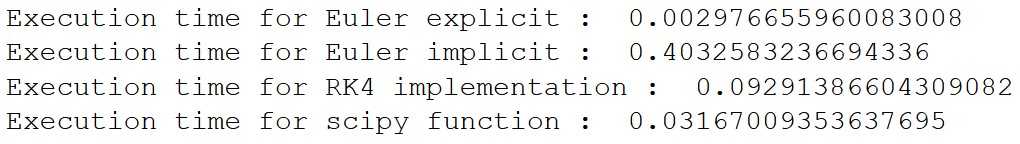
\includegraphics[width=0.7\textwidth]{"images/execution_times.jpg"} \\
		It seems that the explicit Euler method is the fastest, followed by the scipy function. \\
		We can see that implicit Euler is longer than the others. This is probably due to the loop on k for each n. \\
	\end{enumerate}

	\noindent For the next part of the project, we choose to work with the scipy function because as we see before, we don't have to chosse the number of discretization points $N$. Before using this function in more complex case, it can be usefool to understand how it works.
		
	\newpage
	
	\section{Gantt chart}
	\label{diag}
	
	\centering
	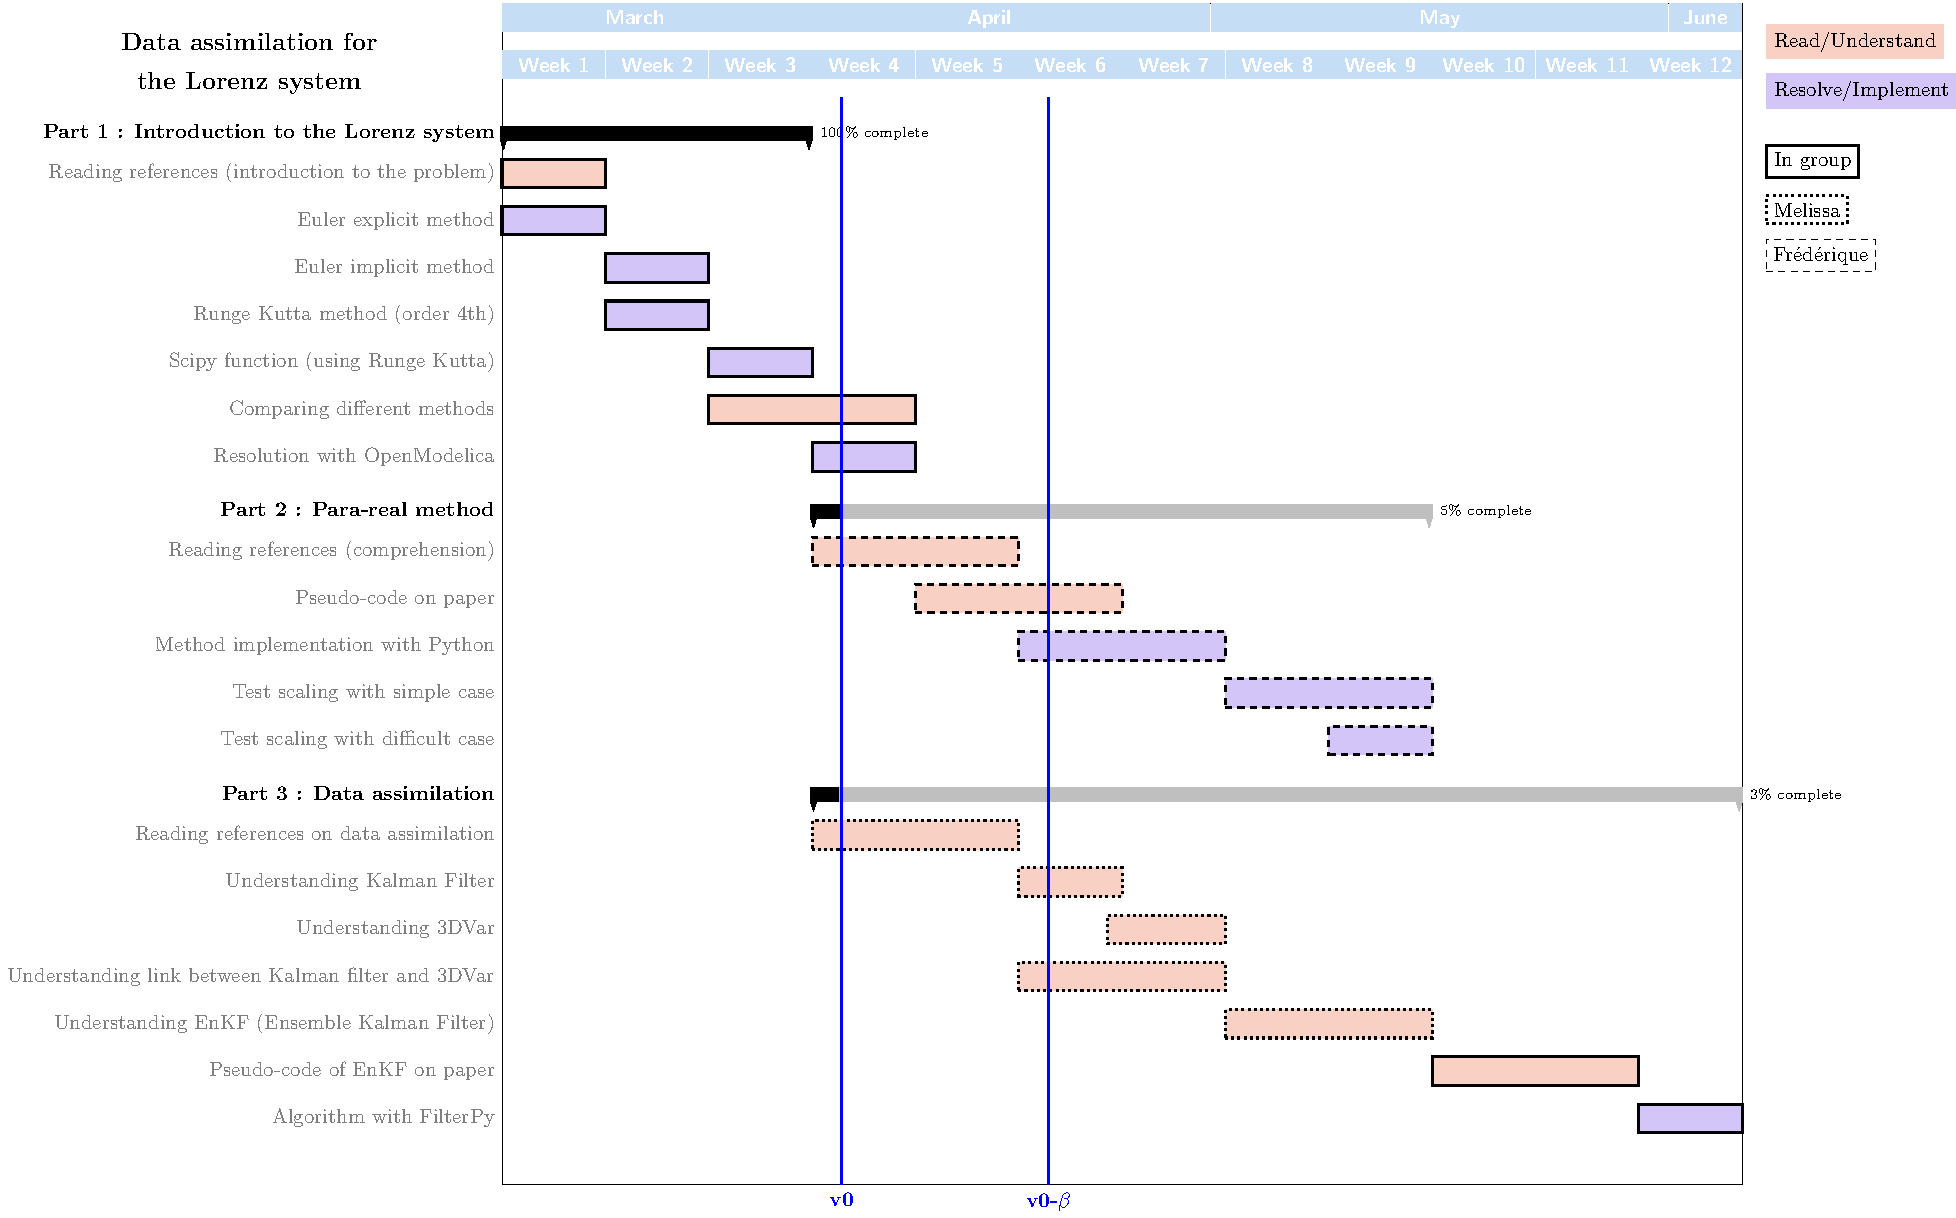
\includegraphics[angle=90,width=0.78\textwidth]{gantt.pdf}
	
	\newpage	
	\bibliographystyle{plain}
	\bibliography{biblio}
	
\end{document}